% arara: pdflatex
% arara: pdflatex
% arara: pdflatex

% options:
% thesis=B bachelor's thesis
% thesis=M master's thesis
% czech thesis in Czech language
% slovak thesis in Slovak language
% english thesis in English language
% hidelinks remove colour boxes around hyperlinks

\documentclass[thesis=B,czech]{FITthesis}[2019/12/23]

\usepackage[utf8]{inputenc} % LaTeX source encoded as UTF-8

\usepackage[T1]{fontenc}

% \usepackage{amsmath} %advanced maths
% \usepackage{amssymb} %additional math symbols

\usepackage{dirtree} %directory tree visualisation

% % list of acronyms
% \usepackage[acronym,nonumberlist,toc,numberedsection=autolabel]{glossaries}
% \iflanguage{czech}{\renewcommand*{\acronymname}{Seznam pou{\v z}it{\' y}ch zkratek}}{}
% \makeglossaries

\newcommand{\tg}{\mathop{\mathrm{tg}}} %cesky tangens
\newcommand{\cotg}{\mathop{\mathrm{cotg}}} %cesky cotangens

% % % % % % % % % % % % % % % % % % % % % % % % % % % % % % 
% ODTUD DAL VSE ZMENTE
% % % % % % % % % % % % % % % % % % % % % % % % % % % % % % 

\department{Katedra informační bezpečnosti (KIB)}

\title{Kubernetes klastr pro lámání hesel}

\authorGN{Tomáš} %(křestní) jméno (jména) autora

\authorFN{Klas} %příjmení autora

\authorWithDegrees{Tomáš Klas} %jméno autora včetně současných akademických titulů

\author{Tomáš Klas} %jméno autora bez akademických titulů

\supervisor{Ing. Jiří Buček, Ph.D. }

\acknowledgements{Doplňte, máte-li komu a za co děkovat. V~opačném případě úplně odstraňte tento příkaz.}

\abstractCS{Hlavní náplní práce je nakonfigurování klastru pro lámání hesel. Tento klastr je řízen pomocí technologie Kubernetes. Program využívá ke své správné funkcionalitě kontejnery. Tyto kontejnery jsou tzv. Docker kontejnery. Použité technologie jsou v práci detailně popsány a rozebrány. Dále se práce zabývá rešerží ukládání hesel v současných systémech a tím jak hesla vypadají. Na závěr na klastru bude proveden test různých metod pro lámání hesel. Tyto metody budou popsány a bude analyzováno, jak je klastr efektní a výkonný pro daný typ lámání. }

\abstractEN{The main goal of the thesis is to setup a cluster managed by kubernetes for password recovery. Next step is to describe used technologies as Docker, Ansible and Hashcat. Thesis contains description of how the passwords are stored and most known attacks to crack them. Successful deployment and password cracking leads to analyzing speed of the cluster and the particular cracking method. }

\placeForDeclarationOfAuthenticity{V~Praze}
\declarationOfAuthenticityOption{4} %volba Prohlášení (číslo 1-6)

\keywordsCS{Kubernetes, Ansible, klastr, Docker, distribuované lámání, hesla, hashcat, nasazení.}

\keywordsEN{Kubernetes, Ansible, cluster, Docker, distributed cracking, passwords, hashcat, deployment.}

% \website{http://site.example/thesis} %volitelná URL práce, objeví se v tiráži - úplně odstraňte, nemáte-li URL práce

\begin{document}

% \newacronym{CVUT}{{\v C}VUT}{{\v C}esk{\' e} vysok{\' e} u{\v c}en{\' i} technick{\' e} v Praze}
% \newacronym{FIT}{FIT}{Fakulta informa{\v c}n{\' i}ch technologi{\' i}}

\begin{introduction}
	%sem napište úvod Vaší práce
\end{introduction}

\chapter{Cíl práce}


\section{Kubernetes}

Jméno Kubernetes pochází z Řecka a znamená to kormidelník. Projekt zložili Joe Beda, Brendan Burns, a Craig McLuckie,ke kterým se rychle připojili inženýři z Googlu, jako Brian Grant a Tim Hockin. Software byl vydán v roce 2014.

Kontejnery jsou perfektní způsob, jak vytvářet aplikace tak, aby byly lehce rozšiřitelné a dobře spravovatelné. Kubernetes nám následné pomáhá k jejich nasazení a škálování. Co všechno tedy Kubernetes dokáží:

%https://kubernetes.io/docs/concepts/overview/what-is-kubernetes/

\begin{itemize}
  	\item \textbf{Service discovery and load balancing}: Kubernetes propojují kontejnery zkrze DNS a nebo jejich IP adresy. Pokud na jeden 	kontejner jde mnoho požadavků, přesměrují tyto požadavky na jiný a tímto způsobem balancují provoz a zajišťují stabilitu aplikace.
	\item \textbf{Orchestrace úložiště}: Dovolují automaticky připojovat vzdálené nebo lokální úložiště do klastru a zajistit tak konzistenci dat, zálohu a vysokou dostupnost z více míst.
  	\item \textbf{Automated rollouts and rollbacks}: Můžeme popsat požadovaný stav pro naše nasazené kontejnery pomocí Kubernetes a ty automaticky a s kontrolou zajistí tento stav. Můžeme například automatizovat vytváření nových kontejnerů, smazání starých a převzetí všech zdrojů jako jsou data a další novým kontejnerem.
	\item \textbf{Automatic bin packing}: Předáme Kubernetes vztvořený klastr s uzly a specifikujeme zdroje, které každý kontejner potřebuje pro své správné fungování. Kubernetes se následně postará o nejlepší rozdělení kontejnerů na uzly tak, aby optimalizoval naše zdroje. To se může nejvíce hodit na cloudových řešení, kde se platí za to, kolik se využívá zdrojů. 
   	\item{Self-healing}:	Kubernetes restartují kontejnery, které selžou, nahradí je, zahodí pokud přestanou odpovídat na specifikované health checky a přestane je nabízet klientům nebo jiným službám dokud nejsou připravené. 
	\item \textbf{Secret and configuration management}: Kubernetes napomáhají ukládání a sdílení či měnění citlivých informací zkrze klastr. Při změně těchto informací tedy nemusíme znovu vytvářet kontejnery a nově všechno předělat. A to bez jejich zveřejňování v konfiguracích. 

\end{itemize}

\subsection{Stavební kameny Kubernetes}

V momentě kdy nasadíme Kubernetes, dostaneme klastr, který se skládá z výpočetních uzlů. Takovému uzlu se říká node a na něm se spouští kontejnerizované aplikace. Každý klastr se skládá z alespoň jednoho takového nodu. 

Tyto výpočetní nody poskztují prostor pro pody. Pod si můžeme představit jako balík, ve kterém jsou umístěné kontejnery. V praxi je nejčastěji Control Plane rozdělen na více počítačů, aby se zajistila vysoká dostupnost a maximalizovala se odolnost proti chybám. 

\begin{figure}[!h]
	\centering
 	\includegraphics[width=0.8\textwidth, angle=0]{kubernetes-architecture.png}
 	\caption[Komponenty Kubernetes]{Komponenty Kubernetes}\label{fig:float}
\end{figure}

\subsubsection{Control Plane}

Součásti Control plane řídí a rozhodují co se stane s klastrem, např. řídí plánování, detekci a odpovědi klastru na události, jako jsou start nového podu pokud není splněn požadovaný stav. 

Komponenty Control plane mohou být spuštěny na jakémkoliv počítači v klastru. Pro jednoduchost jsou však skripty napsané tak, aby tyto komponenty byly spuštěny na jednom počítači. Samotná aplikace je pak směřována mimo tento počítač. 

% https://github.com/etcd-io/etcd
\begin{itemize}
	\item \textbf{kube-apiserver}: Tato komponenta poskytuje API uživateli. Je to front end pro Control plane. Hlavní implementací je kube-apiserver, ten je navržen, aby se dokázal horizontálně škálovat, to znamená, že se dokáže replikovat do více instancí. Můžeme tedy spustit více instancí a balancovat provoz. 
	\item \textbf{etcd}: Skládá se z vysoce dostupné databáze s klíčem a hodnotou pro Kubernetes a všechna klastrová data. Její důležité vlastnosti jsou: jednoduchost, bezpecnost, rychlost, spolehlivost. 
	\item \textbf{kube-scheduler}: Tato komponenta kontroluje a vytváří nové pody, pro které zatím nebyl přiřazen žádný node. Je odpovědná za přiřazení takového podu na nějký node podle požadavků. Vždy musí brát v potaz zdroje, které jsou nutné, hardwarové a softwarové vazby, affinity a anti-affinity specifikace, kde jsou uložena data, vnitřní vytížení a časové termíny.
	\item \textbf{kube-controller-manager}
\end{itemize}

\subsubsection{Pod}



\subsubsection{Plánovač}



\subsubsection{Controller Manager}



\subsubsection{API server}



\subsubsection{Kubelet}



\subsubsection{Kube-Proxy}



\subsection{Kubernetes a tajemství}



\subsection{Aktualizace obraz}



\subsection{Sdílené datové prostory}



\subsection{Cloudový poskytovatelé}





\section{Ansible}

Ansible je automatizační nástroj pro konfiguraci systému, nasazení softwaru, aktualizac. Jeho nejsilnější stránka je nulové výpadky systému při aktualizaci balíčků, nebo automatické nastavovat dané zařízení. 

Jeho hlavními cíly jsou jednoduchost a nenáročnost. Kód by měl být čitelný i pro lidi, kteří nejsou obeznámeni s programem. Je schopen pokrýt různě velké prostředí od malých podniků až po velice obsáhlou infrastrukturu. 

Ansible se připojí na vzdálený počítač pomocí OpenSSH pomocí uživatele, který je současně přihlášen. Na spravovaném počítači není trřeba žádný agent. Je možnost nakonfigurovat Ansible, aby pro připojení nepoužíval OpenSSH, ale i kerberos nebo LDAP. 

Ansible a jemu podobné nástroje se použijí v případě toho, že máme více serverů, nebo pokud budeme dodržovat trend IaaS. Kdyby měl admin ve firmě nasazovat nebo aktualizovat například sto počítačů, tak na každém stráví 15 minut. To bude 1500 minut a to je 25 hodin. Proto použije Ansible a za 20 minut je hotov. 

Pro příklad budeme instalovat Docker na 3 počítače. Na těchto počítačích budeme mit v souboru /root/.ssh/authorized_keys naše veřejné klíče pro ssh. Na hostovi, ze kterého budeme instalovat je potreba Ansible. Tedy "sudo apt install ansible". V souboru hosts, který je pro Ansible tzv. inventářem naspecifikujeme stanice, na které budeme instalovat Docker. 

IP ansible_user=root
IP ansible_user=root
IP ansible_user=root

V souboru deployment.yml se specifikuje, co se bude spouštět a na jakých stanicích. 

= hosts: all
..
..


Ve složce tasks dale napíšeme script, který se spustí pomocí pythonu a jeho modulů na vzdálené stanici.

- name 
  apt"
  	instal: docker.io
  	
  	
  	

\subsection{Komponenty}

\subsubsection{Control node}

Jakýkoliv počítač s nainstalovaným Ansible a pythonem, může spouštět příkazy nebo tzv. playbooky. Tento počítač se nazývá control node. Takových můžeme mít klidně více, ne však počítače, které mají nainstalovaný operační systém Windows. 

\subsubsection{Managed node}

Je jakékoliv síťové zařízení. Managed nodes můžeme také nayývat jako hosts. Tyto zařízení nemusejí mít nainstalovaný Ansible, ale musejí mít nainstalovaný python. Ansible může být nakofigurován, aby používal specifikovanou verzi pythonu, pokud není specifikována, spustí se na hostu jeho defaultní.

\subsubsection{Iventory}

Je seznam všech nastavovaných zařízení. Často se nazývá hostfile. v tomto souboru nastavujeme skupiny zařízení, jejich IP adresy a další specifikace, například jaký python má daný host použít. 

\subsubsection{Modules}

Jsou to jednotlivé části kódu, které bude Ansible spouštět. Každý modul má speciální použití. Vše od správy uživatelů ( user ) přes nastavení systému ( systemd ) až k instalovaní balíčků ( apt, yum ). Můžeme spustit jeden modul v tasku, nebo více v playbooku. Pro přehlednost neuvádím všechnz možné moduly, jelikož je jich přes tři tisíce. 

\subsubsection{Tasks}

Jsou jednotky, které se museji provést. Nejčasteji specifikované v deployment souboru. 

\subsubsection{Playbooks}

Je seřazený seznam tasků, které se musí vykonat. Ničemu neuškodí pokud se plazbook spustí znovu, protože Asnible skontroluje stav daného tasku. Playbooky jsou psané podle konvenci YAMLu. 


\section{Docker}

Docker je otevřená platforma pro vývoj, dodání a spouštění aplikací. Umožnuje oddělení aplikací od infrastruktury, tedy můžeme dodávat software rychleji a bez problémů, které se váží k různorodosti prostředí, ve kterém aplikace běží. Svou fylozofií jsou velice podobné virtualním počítačům. Rozdíly mezi těmito různými pohledy na věc budou rozebrány dále v textu. 

Docker zprostředkovává platformu pro zabalení aplikace i se všemi jejímy závislostmi. Izoluje danou aplikaci od ostatních běžících procesů na daném počítači a zajišťuje tak její bezpečí. Docker kontejner je velice nenáročný na hardware, můžeme jich tedy na daném počítači spustit velice mnoho.  

Fylosofie kontejnerů je taková, že každý kontejner je odpovědný pouze za jednu danou část aplikace. Pro příklad máme naší webovou aplikaci. Budeme tedy mít alespoň tři docker kontejnery. Jeden na kterém poběží NGINX a bude zprostředkovávat naší aplikaci uživatelům. Další bude mít naší aplikaci a ve třetím poběží databáze. 

Konterjnery fungují tedy jako malé počítače, mají izolované veškeré svoje systémové zdroje ( paměť, procesy, internetové rozhraní ). Díky tomuto mohou být rychle a jednoduše přidány, nebo odebrány.  


\subsection{Konterjner vs. virtuální počítač}

Virtualizace je odpověď na problém různorodých prostředí mezi vývojáři a zákazníky. Problém ,který virtualizace a kontejnerizace především řeší je různorodost prostředí mezi zákazníkem a dodavatelem softwaru. Při jeho předávání dochází ke změně prostředí, jsou nainstalované jiné verze závislostí a operačního systému a aplikace se může chovat neočekávaně. 

Podíváme se jak se tyto dvě technologie liší a proč se svět žene právě směrem kontejnerizace, když zde již je řešení.

Virtuální počítač je regulérní stroj, který běží na daném hostovi. Tento stroj má svůj kernel, svůj operační systém a ke zdrojům přistupuje přes tzv. hypervizor např.: QEMU, nebo VirtualBox. Hypervizor zprostředkovává přístup virtuálního stroje k systémovým zdrojům. 

Pro to, aby na hostovi, nebo-li na systému, který má nainstalovaný hypervizor mohlo běžet více virtuálních strojů stačí jedna jeho instance. Nevýhoda tohoto řešení je taková, že se mnoho zdrojů duplikuje. Řekněme, že na hostitelském systému poběží tři aplikace. Každá taková aplikace bude izolovaná od ostatních pomocí virtuálního stroje. Dejme tomu, že to bude databáze, webový server a stroj pro vzdáleného uživatele. Níže uvidíme nákres tohoto řešení. 

% https://www.docker.com/resources/what-container
\begin{figure}[!h]
	\centering
	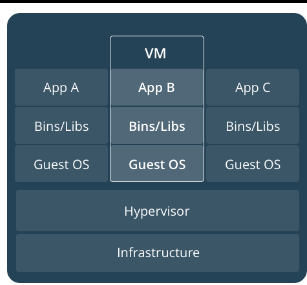
\includegraphics[width=0.73\textwidth, angle=0]{docker-VM.png}
	\caption[Docker VM]{Oddělení aplikací za pomoci hypervizoru a virtuálních strojů.}
	\label{fig:docker-vm}
\end{figure}

To samé, jako je na obrázku výše se pokusíme realizovat pomocí Dockeru a kontejnerů. Kontejnery, jelikož využívají overlayFS jsou schopny poskytnout jádro operačního systému kontejneru bez zbytečné kopie a využívají copy-on-write funkcionality. Níže uvidíme jak za pomoci jmenných prostorů, kontrolních skupin a overlayFS je tento přístup úspornější a rychlejší než virtualizace. 


\begin{figure}[!h]
	\centering
	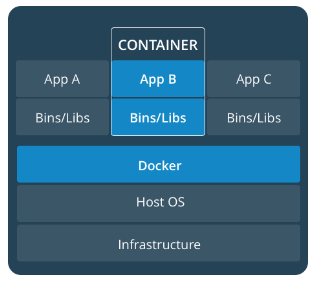
\includegraphics[width=0.8\textwidth, angle=0]{docker-docker.png}
	\caption[Docker kontejnery]{Oddělení aplikací za pomoci Dockeru}
	\label{fig:docker-docker}
\end{figure}

Místo, které jsme na hostitelském systému ušetřili však není jediná výhoda. Na tomto příkladu se však rozdíly mezi těmito technologiemi vysvětlují nejlépe. Dalšími výhodami je rychlost spuštění kontejneru a virtuálního stroje. Při spuštění se pouze připojí obraz OS, vytvoří se izolované procesy a popřípadě se omezí i zdroje, které má kontejner využívat. Nehledě na to, že pokud kontejner nemá omezení nebo limit využitých zdrojů alokuje si je dynamicky oproti virtuálnímu počítači, který si pro sebe naalokuje danou paměť při spuštění.  


\subsection{Stavební kameny Dockeru}

Jak je již uvedeno v předešlé kapitole, Docker využívá vychytávky linuxového kernelu pro svojí funkcionalitu. Díky tomuto perfektně funguje na počítačích, kde běží OS založený na Linuxu. V následujících sekcích budou tyto technologie blíže popsány a bude vysvětlena jejich důležitost. 

\begin{figure}[!h]
	\centering
	\includegraphics[width=0.8\textwidth, angle=0]{docker-architecture.png}
	\caption[Docker architektura]{Docker a jeho komponenty.}
	\label{fig:docker-architecture}
\end{figure}

%TODO Jak jsou na tom jiné OS

\subsubsection{Jmenné prostory}

Jmenné prostory zastřešují veškeré zdroje systému tak, že každý proces spuštěn v daném prostoru může používat pouze prostředky, které se váží k tomuto prostoru. Každému procesu se to jeví tak, že má svoje vlastní globální prostředky, které mohou vidět i ostatní procesy z jmenného prostoru, ale ne z jiného. V tabulce \ref{tab:Jmenne prostory} je možné videt, jaké jmenné prostory lze v Linuxu nalézt.

% parametry pro table: h! = nejblize
% p{5cm} na zalomovani bunky
\begin{table}[h!]
  \begin{center}
	\caption{Linuxové jmenné prostory}
    \label{tab:Jmenne prostory}
    \begin{tabular}{|l|l|} 
    	  \hline
      \textbf{Jméno} & \textbf{Popis} \\
      \hline

	  Cgroup  &  Cgroup root adresář\\
	  IPC     &  Systém pro komunikaci procesů, POSIX fronty\\
	  Network &  Síťové rozhraní, protocoly, porty, etc\\
      Mount   &  Připojená zařízení\\
      PID     &  ID procesů\\
      User    &  Uživatelská ID a ID skupin\\
      UTS     &  Hostname a NIS doménu\\   
      
      \hline
    \end{tabular}
  \end{center}
\end{table}

Při spuštění kontejneru dojde k vytvoření procesu na hostitelském systému. Procesy dostanou od systému nějaké PID a chovají se jako normální procesy. Pokud se však přihlásíme do kontejneru (command: docker exec -it name bash) a podíváme se na procesy běžící v daném kontejneru uvidíme, že procesy mají jiná PID a určitě mají i PID=1. Toto nám umožňují jmenné prostory.

Každý kontejner může mít svůj vlastní souborový systém a svoje síťové rozhraní. Vše co můžeme oddělit mezi hostitelem a kontejnery je uvedeno v tabulce výše. 

\subsubsection{Kontrolní skupina}

Je to vlastnost Linuxového kernelu. Jejich hlavní funkcí je limitovat zdroje. V Dockeru se používají protože dovolují sdílet prostředky mezi hostitelským systémem a dalšímy kontejnery. 

Často dochází k záměně pojmů mezi kontrolními skupinami a jmennými prostory. Znovu to tedy shrňme. Kontrolní skupinz, nebo-li cgroups omezují co můžeme použít a jemenné prostorz nebo-li namespaces omezují co jsme schopni vidět v systému. 

\subsubsection{Docker daemon}

Docker daemon nebo-li dockerd poslouchá dotazy na docker API a spravuje objekty jakou jsou docker obrazy, kontejnery, síť a úložiště. Komunikuje ale i s dalšími daemony, aby byl schopen řídit službu Docker.

\subsubsection{Docker klient}

Je to primární cesta, jak komunikovat s Dockerem. Když použijeme příkazy, jako jsou "docker run", klient odešle příkazy daemono zmíněného výše. 

\subsubsection{Docker registr}

Docker registr je úložiště pro naše Docker obrazy. Bez předchozího nastavení hledá dockerd obrazy, které chceme spustit ve veřejném Docker registru. Obrazy však mohou být dostupné i lokálně, nebo na nějaké jiné službě, např.: gitlab container registry. 

Do styku s registrem přícházíme hlavně ve chvílích, kdy provádíme příkazý docker pull, docker push a docker run. Tyto příkazy vždy potřebují znát obraz, který bude spouštěn jako základní vrstva pro nový kontejner, nebo bude stáhnut na lokání počítač, či nasdílen do registru.

\subsubsection{Obrazy}

Můžeme si to představit jako šablonu, na které je spuštěn kontejner. Obraz může být složen z vícero obrazů, nebo z nich vycházet. 

Pro vytvoření obrazu je třeba soubor Dockerfile. Tento soubor obsahuje jednoduché kroky, které je třeba vykonat pro vytvoření konkrétního obrazu. Např.: jaké použijeme a zveřejníme porty, jaké balíčky chceme ve vytvořeném obrazu mít atd. 

Každý příkaz v Dockerfilu vytvoří na locálním počítači tzv. vrstvu, kterou při úpravě Dockerfilu mění nebo předělává pouze pokud byla změněna. 

%TODO picture of docker architecture

\subsection{Systémová kontejnery}

Docker kontejnery nejsou však jediné, které se v produkčním prostředí používají. Patří do tzv. aplikačních kontejnerů. Jejich účel je zpravidla spouštět pouze jeden proces. K takovýmto kontejnerům můžeme ještě přidat kontejnerz Rocket. Hlavním rozdílem je to, že rtk nemá na systému spuštěného daemona jako má např. Docker. Při spuštění se tedy pod běžícím spustí další. 

Dále tady máme systémové kontejnery. Ty jsou používané jako klasické OS. Na jednom silném stroji může běžet několik takových kontejnerů a ty mohou uživateli poskytovat oddělené prostředí od celého serveru a nabídnout mu izolovaný prostor od ostattních pomocí výše zmíněných technologií. Tuto možnost zastřešuje projekt LXC později LXD.

%TODO add image of the lxc list



\subsection{Proč použít Hashcat?}

\chapter{Hesla}

Hesla můžeme vidět všude a ne jen v informatice. 
Pokud se podíváme zpět do historie např. do doby velkého Caesara a jeho šifry, ke které je třeba znát číslo, o které se posouvají znaky ve zprávě. 
Jak tedy můžeme vidět, hesla neslouži pouze k naší autentizaci vůči nějaké službě či serveru. 
Může je také použít k podepsání citlivých dokumentů jako je třeba příloha e-mailu. 
Následně pak nemůžeme popřít jeho poslání. Tomuto se říká elektronický podpis. 

Hesla však mají nejednu nevýhodu. Útočník může s naším nebo i bez našeho vědění odhalit naše heslo a tím nám narušit naše soukromý. Hesla mohou také být v systémech, které používáme uložena nepatřičným způsobem, jako je například čistý text bez použití žádných ochranných prostředků. 

Hesla též mohou ze systému uniknout. V tomto případě, pokud byla hesla uložena neptřičným způsobem nemusí se potencionální útočník nějak přemáhat, aby uživatele kompromitoval. Proto se zaměříme na to jak mohou a jak skutečně jsou uložena v nejpoužívanějších systémech. 

\section{Hašovací funkce}

Jsou to takové funkce f: X ® Y, pro něž je snadné z jakékoli hodnoty x Î X vypočítat y = f(x), ale pro náhodně vybraný obraz y Î f(X) nelze v relevatním čase najít její vzor x Î X tak, aby y = f(x).

Přitom víme, že takový vzor existuje nebo jich existuje dokonce velmi mnoho. To kolik jich existuje se odvíjí jakou hašovací funkci použijeme.

\subsection{Vlastnosti hašovací funkce}

Abychom mohli funkci považovat za hašovací, musí mít následující vlastnosti:

\begin{itemize}
    \item jakékoliv množství vstupních dat poskytuje stejně dlouhý výstup (otisk),
    \item malou změnou vstupních dat dosáhneme velké změny na výstupu,
    \item z hashe je prakticky nemožné rekonstruovat původní text zprávy,
    \item v praxi je vysoce nepravděpodobné, že dvěma různým zprávám odpovídá stejný hash, jinými slovy pomocí hashe lze v praxi identifikovat právě jednu zprávu (ověřit její správnost).
\end{itemize}

%TODO narozeninovy paradox a projit si prezentace na bezpecnost o hashich

\subsection{Naorzeninový paradox}



\subsection{Windows}

Windows se chovají jinak v doméně a jinak mimo ní. Pokud je počítač v doméně je preferován autentizační protokol kerberos. V současných Windows Server edicích je implementován Kerberos verze 5. Kerberos v základní nastavenim operuje na portu 88 a k šifrování používá symetrickou šifru. 
Pokud počítač není nastaven aby se autentikoval pomocí protokolu Kerberos používají Windows šifrování NTLM.

\subsection{Linux}

Hesla v linuxových systémech se skládají ze dvou konkretních souborů. 

/etc/shadow - obsah a strukturu toho souboru můžeme vidět na následujícím obrázku. 

% TODO Pictore of the structure  

/etc/passwd - obsah a strukturu tohoto souboru můžeme vidět na následujícím obrázku.

% TODO Pictore of the structure 

V /etc/shadow jsou hesla uložená pomocí hashe. 

\subsection{MacOS}

%TODO MacOS password handling

\section{Útoky na hesla}

\subsection{Hrubou silou}

\subsection{Pomocí masky}

\subsection{Se slovníkem}

\section{Entropie hesla}

\section{Ochrana před různými útoky}



% \input{realizace}

\chapter{Závěr}
\cite{merkel2014docker}
test
	
% TODO get csns690
%\bibliographystyle{csn690}
\bibliographystyle{ieeetr}

\bibliography{mybibliographyfile}

\appendix

\chapter{Seznam použitých zkratek}
% \printglossaries
\begin{description}
	\item[GUI] Graphical user interface
	\item[XML] Extensible markup language
\end{description}



\chapter{Obsah přiloženého CD}

%upravte podle skutecnosti

\begin{figure}
	\dirtree{%
		.1 readme.txt\DTcomment{stručný popis obsahu CD}.
		.1 exe\DTcomment{adresář se spustitelnou formou implementace}.
		.1 src.
		.2 impl\DTcomment{zdrojové kódy implementace}.
		.2 thesis\DTcomment{zdrojová forma práce ve formátu \LaTeX{}}.
		.1 text\DTcomment{text práce}.
		.2 thesis.pdf\DTcomment{text práce ve formátu PDF}.
		.2 thesis.ps\DTcomment{text práce ve formátu PS}.
	}
\end{figure}

\end{document}

